\documentclass{article}
\usepackage{graphicx}
\usepackage{hyperref}
\usepackage{minted}

\title{WiCyS CTF 2023 Weird Sounds Writeup}
\author{Manav Malik}
\date{}

\begin{document}

\maketitle

We begin, as always, by examining the challenge description:

\begin{quote}
    I found a really weird audio file that apparently has some kind of message encoded in it. Can you find it?
\end{quote}
The audio in question is a {\sf .wav} file. Taking a quick listen to the various blips and bloops does not yield any helpful information. A common red herring might be to try to interpret the audio as Morse code, but following this path quickly shows that this is not the solution. Instead, we can take the audio and stick it in Audacity. The default view shows the audio's waveforms, but showing the spectrogram view yields the flag.
\begin{figure}
    \centering
    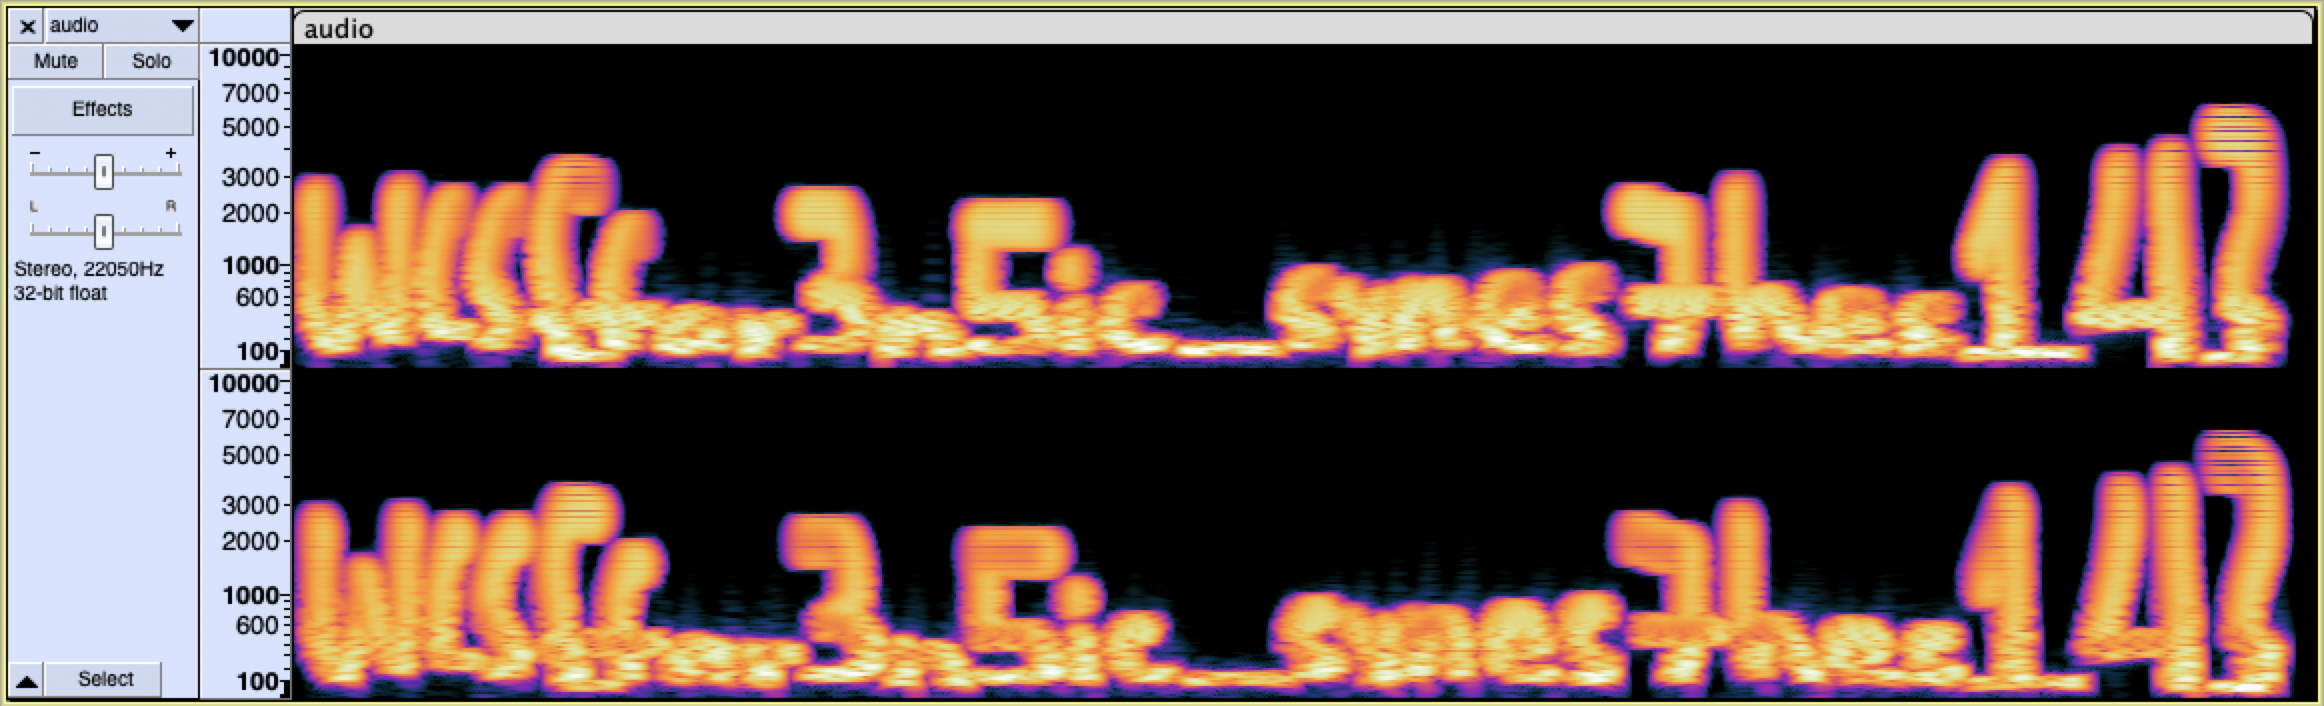
\includegraphics[width=\linewidth]{writeup_ss.png}
    \caption{Screenshot of spectrogram view in Audacity}
    \label{fig:flag-ss}
\end{figure}
Our flag is: {\sf WCS\{for3n5ic\_synes7hes14\}}

\end{document}
